% MAT670 -- Lecture XI (scans MAT670_XI, pp. 1--14)
\chapter{Lecture 11: Critical points, jamming and entropy}
\label{L11:ch}

\section{Critical points and jamming}
\label{L11:sec:critical}

\added{Throughout, a configuration is an ordered $N$-tuple $X=(x_1,\dots,x_N)$ of points on the sphere $\Sph^2$, and $d$ denotes the geodesic (angular) distance. Let $f(X)=\min_{i<j}d(x_i,x_j)$ and write $\Conf(N;\theta)=\{X: f(X)\ge\theta\}$. A configuration in $\Conf(N;\theta)$ is the same thing as a packing of $N$ spherical caps of angular radius $\rho=\theta/2$.}

Last time we stated the following theorem, which characterizes the regular values of $f$ in terms of the geometry of the contact graph.

\begin{definition}[Contact graph]\label{L11:def:contact}
Let $X\in\Conf(N;\theta)$ with $f(X)=\theta$, where $\theta=2\rho$. The \emph{contact graph} of $X$ is the set of edges on $\Sph^2$ \added{(geodesic arcs)} joining those points $x_i,x_j$ that are at distance exactly $\theta$.
\end{definition}
\orig{crossed out: ``geodesic skeleton of'', ``struts''}

\begin{addedblock}
For an edge $\{i,j\}$ of the contact graph let $u_{ij}\in T_{x_i}\Sph^2$ be the unit tangent vector at $x_i$ pointing along the geodesic towards $x_j$ (well defined since $0<\theta<\pi$). A tangent vector $v=(v_1,\dots,v_N)$, $v_i\in T_{x_i}\Sph^2$, changes the length of the edge at rate
\[
\frac{d}{dt}\Big|_{t=0} d(x_i+tv_i,\,x_j+tv_j) \;=\; -\ip{u_{ij}}{v_i}-\ip{u_{ji}}{v_j}.
\]
We say $v$ lies in the \emph{tangent cone} (of increasing directions) at $X$ if this rate is strictly positive for every contact edge, and that $\theta$ is a \emph{regular value} of $f$ if every $X$ with $f(X)=\theta$ admits such a $v$; otherwise $\theta$ is a \emph{critical value} and the offending $X$ are \emph{critical configurations}.
\end{addedblock}

\begin{theorem}\label{L11:thm:forcebalance}
A configuration $X$ with $f(X)=\theta$ has no element in its tangent cone if and only if there exist weights $w_{ij}=w_{ji}\ge0$ on the contact edges, not all zero, such that the contact graph is \emph{force balanced}:
\[
\sum_{j:\,\{i,j\}\text{ contact}} w_{ij}\,u_{ij} \;=\; 0 \qquad\text{for every vertex } i.
\]
In particular, $\theta$ is a regular value if and only if no configuration at level $\theta$ admits such a balanced (non-negative, not all zero) system of weights.
\end{theorem}
\orig{``(non-negative, not all 0)'' replaces crossed-out ``(positive)''}

\begin{addedblock}
\emph{Proof sketch.} Let $A$ be the linear map $v\mapsto\big(-\ip{u_{ij}}{v_i}-\ip{u_{ji}}{v_j}\big)_{\{i,j\}}$ from $\bigoplus_i T_{x_i}\Sph^2$ to $\R^{E}$, $E$ the set of contact edges. By Gordan's alternative (a form of Farkas' lemma), either there is $v$ with $Av>0$ componentwise, or there is $w\in\R^E$, $w\ge0$, $w\ne0$ with $A^{T}w=0$. Computing $A^Tw$ vertex by vertex gives exactly $-\sum_j w_{ij}u_{ij}=0$. Together with the deformation theorem from last lecture (if $[a,b]$ contains no critical values, then $\Conf(N;b)$ is a deformation retract of $\Conf(N;a)$), this is the basic tool for computing the topology of $\Conf(N;\theta)$ as $\theta$ increases.
\end{addedblock}

The simplest application is to points on a circle.

\begin{theorem}\label{L11:thm:circle}
\added{For $N$ points on the circle $\Sph^1$,} $\Conf(N;0)\simeq\Conf(N;2\pi/N)$.
\end{theorem}
\unclear{Blotted symbol before $2\pi/N$; read here as the circle case. Possibly ``$<$'': the $\Sph^2$ theorem, see remark.}
\begin{addedblock}
\emph{Alternative reading.} The blot may be ``$\theta<$'', i.e.\ the statement for $\Sph^2$:
$\Conf(N;\theta)$ is a strong deformation retract of $\Conf(N;0)$ for $0\le\theta<2\pi/N$. This is
Theorem~4.14 of Kusner--Kusner--Lagarias--Shlosman (cited in \S\ref{L11:sec:examples}). It sharpens
the bound $\pi/N$ of Lecture~10, since a balanced contact graph has total length at least $2\pi$,
and the smallest critical value is attained only by $N$ equally spaced points on a great circle. The
proof sketch below covers only the circle.
\end{addedblock}

\begin{addedblock}
\emph{Proof sketch.} Here $\Conf(N;0)$ means the usual ordered configuration space (distinct points). On $\Sph^1$ the vectors $u_{ij}$ at $x_i$ are $\pm$ the unit tangent, so force balance at a vertex forces it to have one contact on each side with equal weights. Following the weights along a chain of contacts, a chain with an endpoint is unbalanced at that endpoint; hence the contact graph of a critical configuration is the whole $N$-cycle, i.e.\ $X$ is a regular $N$-gon and $\theta=2\pi/N$. Thus there are no critical values in $(0,2\pi/N)$, so $\Conf(N;\theta)\simeq\Conf(N;0)$ for $\theta<2\pi/N$. At $\theta=2\pi/N$ itself the space consists of the labelled regular $N$-gons, a disjoint union of $(N-1)!$ circles (one for each cyclic order of the labels); and $\Conf(N;0)$ has the same homotopy type, each of its $(N-1)!$ components being a circle times an open simplex.
\end{addedblock}

This also gives an algorithm for exploring critical and maximal configurations: \emph{$\rho$-evolution}. Starting from any configuration, increase $\rho$ by moving the points in a direction of the tangent cone; update the contact graph whenever new contacts form, and continue until no increasing direction exists, i.e.\ until the contact graph becomes force balanced.
\unclear{Page ends with ``update\ldots'' and ``conflicting\ldots'' (or ``conf-flip''?); not expanded.}
\added{The configuration reached is then a critical configuration, generically a local maximum of $f$ (a \emph{jammed} configuration).}

\section{Examples with pictures}
\label{L11:sec:examples}

\orig{p.~2: ``$N=3$, $N=4$: full picture'' -- pictures were presumably drawn on the board.}
For $N=3$ and $N=4$ one can give the full picture of the critical points.
\begin{addedblock}
For $N=3$: a vertex with a single contact cannot be balanced, so every vertex of a critical contact graph has degree $2$, and the two tangent vectors at it must be opposite; thus the three points lie on a great circle, equally spaced. The only critical value is the maximum $\theta=2\pi/3$, and $\Conf(3;\theta)\simeq\Conf(3;0)$ for $\theta<2\pi/3$.
For $N=4$: the maximum is the regular tetrahedron, $\theta=\arccos(-1/3)\approx109.47^\circ$. The square inscribed in a great circle ($\theta=\pi/2$) is also critical (each vertex has two opposite contacts), but it is not a local maximum: pushing alternate vertices slightly north and south increases all four contact distances to second order, deforming the square towards the tetrahedron.
\end{addedblock}

For larger $N$:
\begin{itemize}
\item For various $N$ the maximum is the solution of the \emph{Tammes problem}. \added{(The Tammes problem is solved for $N\le 14$ and $N=24$; e.g.\ $N=13$ and $N=14$ by Musin--Tarasov, $N=24$ by Robinson.)}
\item $N=10$: local maxima? \unclear{``$N=10$ -- local max?'': whether there are non-global local maxima, presumably.}
\item $N=12$: local maxima? Higher critical points. The jitterbug?
\end{itemize}
\begin{addedblock}
For $N=12$ the global maximum is the icosahedron ($\theta=\arctan 2\approx63.43^\circ$). The cuboctahedron (the kissing configuration of the FCC lattice, $\theta=60^\circ$) is a critical configuration that is not a local maximum; Buckminster Fuller's ``jitterbug'' motion deforms the cuboctahedron into the icosahedron. (See R.~Kusner, W.~Kusner, J.~Lagarias, S.~Shlosman, \emph{Configuration spaces of equal spheres touching a given sphere: the twelve spheres problem}, arXiv:1611.10297 (2016); in \emph{New Trends in Intuitive Geometry}, Bolyai Soc.\ Math.\ Stud.\ 27, Springer, 2018. That paper shows the cuboctahedral (FCC) configuration is critical. That it is not a local maximum follows from the jitterbug: along it the triangle edges lengthen from $60^\circ$ to $\arctan 2$, while the square diagonals shrink from $90^\circ$ to $\arctan 2$.)
\end{addedblock}

\section{Local maxima and Edwards entropy}
\label{L11:sec:edwards}

\begin{definition}[Edwards' ansatz]\label{L11:def:edwards}
All jammed states of equal volume have equal probability.
\end{definition}
\orig{``Edw.'' crossed out and replaced by ``Ansatz''}
\begin{addedblock}
This is the hypothesis of S.~F.~Edwards and R.~B.~S.~Oakeshott (\emph{Theory of powders}, Physica A, 1989). The \emph{Edwards entropy} at volume $V$ is the logarithm of the number (or measure) of jammed states of volume $V$; it plays the role that the Boltzmann entropy plays for the microcanonical ensemble.
\end{addedblock}

This is related to the evolution of the $\rho$-flow: \added{if configurations are chosen at random and then evolved by $\rho$-evolution, the probability of a given jammed state is the measure of its basin of attraction, and Edwards' ansatz says these basins are (for equal volumes) equally large.} It is also related to the model \ldots\ \unclear{``Also the model\ldots''; crossed out: ``ex.\ annealed''} It is not always true\,? \added{Numerical studies of small disc packings have found that jammed states are in general \emph{not} equally likely, and that the frequencies depend on the preparation protocol.}
\added{\emph{Update:} later work (Martiniani, Schrenk, Ramola, Chakraborty, Frenkel, \emph{Nature Physics}, 2017) gave numerical evidence that the ansatz does hold for soft-sphere packings exactly at the jamming threshold.}

\subsection{Boltzmann measure: the discrete setting}
\label{L11:sec:boltzmann}

Consider $N$ particles, each in one of $k$ states. Each state has an energy $E_i$, $i\in\{1,\dots,k\}$. Let $n_i$ be the number of particles in state $i$. The system is closed, so
\[
E=\sum_{i=1}^k E_i\,n_i,\qquad N=\sum_{i=1}^k n_i
\]
\orig{he writes both $n_i$ and $N_i$; unified to $n_i$}
are fixed. The number of ways to place the particles with occupation numbers $\{n_1,\dots,n_k\}$ is the multinomial coefficient
\[
W=\frac{N!}{n_1!\,n_2!\cdots n_k!}.
\]
By the law of large numbers, the optimal partition (the one maximizing $W$) dominates for $N$ large.
\added{(More precisely: $W$, as a function of the frequencies $n_i/N$, is $e^{N H+o(N)}$ with $H=-\sum (n_i/N)\ln(n_i/N)$, so frequencies whose entropy is smaller than the maximum by a fixed amount are exponentially rare.)}
So we determine the partition that maximizes $W$; since $\log$ is monotone increasing we may replace $W$ by $\log W$. By Stirling's formula,
\[
\log W=(N\ln N-N)-\sum_{i=1}^k\,(n_i\ln n_i-n_i)\;+\;\text{error}\quad\added{(\text{error }=O(k\ln N))}.
\]
We maximize subject to the two constraints with Lagrange multipliers $\alpha,\beta$:
\[
f=\ln W+\alpha\Big(N-\sum_{i=1}^k n_i\Big)+\beta\Big(E-\sum_{i=1}^k E_i n_i\Big).
\]
Since $\frac{\partial}{\partial n}(n\ln n-n)=\ln n$,
\[
0=\frac{\partial f}{\partial n_i}=-\ln n_i-(\alpha+\beta E_i),
\qquad\text{so}\qquad n_i=e^{-\alpha-\beta E_i}.
\]
\added{Summing over $i$ gives $N=e^{-\alpha}Z$, which eliminates $\alpha$:}
\[
\frac{n_i}{N}=\frac{e^{-\beta E_i}}{\sum_{j=1}^k e^{-\beta E_j}},\qquad
Z=\sum_{j=1}^k e^{-\beta E_j}\quad\added{\text{(the \emph{partition function})}}.
\]

\begin{definition}\label{L11:def:boltzmann}
Here $\beta=\dfrac1T$ \ (or $\dfrac{1}{k_BT}$ \added{with Boltzmann's constant $k_B$}) is the inverse temperature, and
\[
F=-T\ln Z
\]
is the \emph{free energy}. The \emph{Boltzmann measure} is
\[
\Pr(\text{state } i)=\frac{e^{-\beta E_i}}{Z}.
\]
\end{definition}

The mean energy per particle is
\[
\bar E=\frac EN=\sum_{i=1}^k E_i\frac{n_i}{N}
=\sum_{i=1}^k\frac{E_ie^{-\beta E_i}}{Z}
=\frac{-\frac{\partial}{\partial\beta}Z}{Z}
=-\frac{\partial}{\partial\beta}\ln Z.
\]
\fixed{page has $e^{\beta E_i}$ and final ``$-\partial_\beta Z$''; signs and $\ln$ corrected}

\begin{lemma}\label{L11:lem:concave}
$-\ln Z$ is concave \added{as a function of $\beta$}. Equivalently, $\bar E=-\frac{\partial}{\partial\beta}\ln Z$ is monotone \added{(non-increasing in $\beta$, i.e.\ non-decreasing in $T$)}.
\end{lemma}
\begin{proof}[Proof idea]
We must show $\dfrac{\partial^2}{\partial\beta^2}\ln Z\ge0$. Why? Write it as the variance of $E$, which is $\ge0$.
\begin{addedblock}
Indeed, with $\langle g\rangle=\sum_i g(E_i)e^{-\beta E_i}/Z$,
\[
\frac{\partial^2}{\partial\beta^2}\ln Z=\frac{Z''}{Z}-\Big(\frac{Z'}{Z}\Big)^2=\langle E^2\rangle-\langle E\rangle^2=\operatorname{Var}(E)\ge0,
\]
with equality only if all $E_i$ are equal.
\end{addedblock}
\end{proof}
\fixed{page has ``$>0$''; it is $\ge 0$}

Thus $-\dfrac1\beta\ln Z$ is the free energy.
\fixed{page: ``$\frac1\beta\ln Z$''; sign restored as in $F=-T\ln Z$}
As $T\to\infty$ (i.e.\ $\beta\to0$), $\Pr(i)\to\dfrac1k$: all states become equally likely. \added{As $T\to0$ the measure concentrates on the states of minimal energy.}

\begin{remark}
\added{For hard particles the energy of a configuration is $0$ if the particles do not overlap and $+\infty$ if they do. The Boltzmann weight $e^{-\beta E}$ is then the indicator of the admissible configurations, so the Boltzmann measure is normalized volume on the configuration space, at every temperature. This is why volumes of configuration spaces appear as partition functions below.}
\end{remark}

\subsection{The hard disc model in an interval}
\label{L11:sec:hardrods}

Place hard discs \added{of diameter~$1$ (that is, hard rods of length~$1$)} in the interval $[0,N]$, and let $a_1,a_2,a_3,\dots$ be the gaps \added{in front of the first, second, third, \ldots\ disc}.

\begin{center}
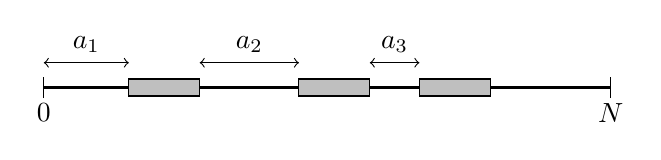
\begin{tikzpicture}[scale=0.9]
\draw[thick] (0,0) -- (8,0);
\draw (0,-0.15)--(0,0.15) node[below=6pt] {$0$};
\draw (8,-0.15)--(8,0.15) node[below=6pt] {$N$};
\foreach \x in {1.2,3.6,5.3} { \fill[gray!50] (\x,-0.12) rectangle (\x+1,0.12); \draw (\x,-0.12) rectangle (\x+1,0.12); }
\draw[<->] (0,0.35) -- node[above] {$a_1$} (1.2,0.35);
\draw[<->] (2.2,0.35) -- node[above] {$a_2$} (3.6,0.35);
\draw[<->] (4.6,0.35) -- node[above] {$a_3$} (5.3,0.35);
\end{tikzpicture}
\end{center}

With three discs the configuration space is
\[
\Omega_{N,3}=\{(a_1,a_2,a_3):\ 0\le a_1,a_2,a_3,\ \ a_1+a_2+a_3\le N-3\},
\]
a simplex \orig{p.~7: sketch of the simplex with axes $a_1,a_2,a_3$} with
\[
\vol\Omega_{N,3}=\frac{(N-3)^3}{3!}.
\]
In general, \added{for $k\le N$ discs,}
\[
\vol(\Omega_{N,k})=\frac{(N-k)^k}{k!}.
\]
\added{(The gaps describe the discs up to relabelling; for labelled discs multiply by $k!$.)}

Now give each particle an energy $E_0$ and define the \emph{fugacity}
\[
z=e^{-\beta E_0}.
\]
\added{(In the usual notation $z=e^{\beta\mu}$ with chemical potential $\mu$; here $\mu=-E_0$.)} The \added{grand canonical} partition function is
\[
Z_N(z)=\sum_{k=0}^N z^k\,\vol(\Omega_{N,k})=\sum_{k=0}^N\frac{(N-k)^k}{k!}\,z^k.
\]
\added{This is the classical \emph{Tonks gas} (L.~Tonks, 1936), one of the few exactly solvable models of hard particles.}

\begin{exercise}\label{L11:ex:tonks}
\added{Using Stirling's formula on the largest term, show that $\frac1N\ln Z_N(z)\to P$, where $P>0$ solves $z=Pe^{P}$, and that the dominant number of discs satisfies $k/N\to P/(1+P)$. ($P$ is $\beta$ times the pressure; note that the density $k/N$ increases from $0$ to $1$ as $z$ goes from $0$ to $\infty$.)}
\end{exercise}

\section{A quasi-one-dimensional model with open ends}
\label{L11:sec:channel}

\orig{crossed out: ``Model''}
We study discs in a narrow channel, where a combinatorial analysis is possible. Take discs of radius $r=1$ in a channel whose width $w$ satisfies
\[
2<w<2+\sqrt3 .
\]
\begin{addedblock}
The centres then lie in a strip of width $h=w-2\in(0,\sqrt3)$. Discs cannot pass each other ($h<2$). If two consecutive discs touch while lying against opposite walls, their centres are horizontally $L=\sqrt{4-h^2}$ apart, and $1<L<2$; the condition $h<\sqrt3$ is exactly $L>1$, which guarantees that each disc can touch only its two neighbours in the row (discs $i$ and $i+2$ are always more than $2$ apart). Consecutive discs touching along the same wall are horizontally $2$ apart.
\end{addedblock}

\begin{figure}[ht]
\centering
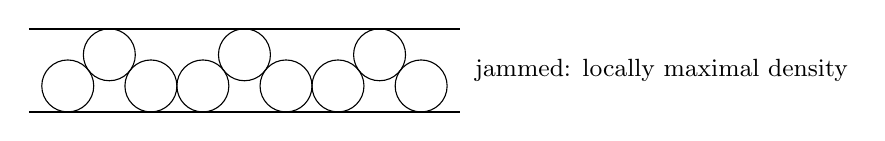
\begin{tikzpicture}[scale=0.33]
% channel width 3.2, h = 1.2, L = 1.6
\draw[thick] (-1.5,0) -- (15.1,0); \draw[thick] (-1.5,3.2) -- (15.1,3.2);
\foreach \x/\y in {0/1,1.6/2.2,3.2/1,5.2/1,6.8/2.2,8.4/1,10.4/1,12.0/2.2,13.6/1} { \draw (\x,\y) circle (1); }
\node[right] at (15.3,1.6) {\small jammed: locally maximal density};
\end{tikzpicture}

\vspace{2ex}
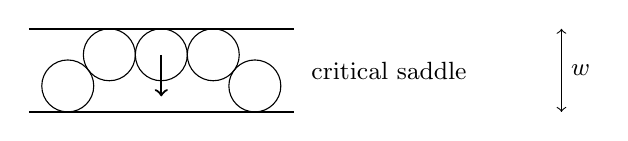
\begin{tikzpicture}[scale=0.33]
\draw[thick] (-1.5,0) -- (8.7,0); \draw[thick] (-1.5,3.2) -- (8.7,3.2);
\foreach \x/\y in {0/1,1.6/2.2,3.6/2.2,5.6/2.2,7.2/1} { \draw (\x,\y) circle (1); }
\draw[->,thick] (3.6,2.2) -- (3.6,0.6);
\node[right] at (9,1.6) {\small critical saddle};
\draw[<->] (19,0) -- node[right] {\small $w$} (19,3.2);
\end{tikzpicture}
\caption{Discs in a narrow channel ($h=1.2$, $L=1.6$). Top: a jammed configuration, contact word $00100100$. Bottom: three consecutive discs on the same wall (word $011\,0$); the middle one is force balanced but can be pushed into the gap, so this is a critical point but not a local maximum.}
\label{L11:fig:channel}
\end{figure}
\orig{p.~9: three sketches; third shows a narrow channel with discs in a staircase}

Let the length of the configuration be $t$. \added{(Discs are confined only by the walls; the ends are open, so ``jammed'' means that $t$ is locally minimal for the given number of discs.)}

\subsection{\texorpdfstring{Combinatorics: how many maxima for given $t$?}{Combinatorics: how many maxima for given t?}}

The length is determined by the number of adjacent pairs of discs at opposite walls \added{versus at the same wall}. Record each contact between consecutive discs by a letter:

\begin{center}
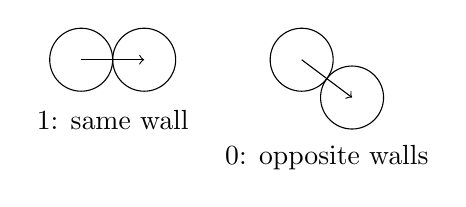
\begin{tikzpicture}[scale=0.4]
\draw (0,0) circle (1); \draw (2,0) circle (1); \draw[->] (0,0)--(2,0);
\node at (1,-1.9) {$1$: same wall};
\draw (7,0) circle (1); \draw (8.6,-1.2) circle (1); \draw[->] (7,0)--(8.6,-1.2);
\node at (7.8,-3.1) {$0$: opposite walls};
\end{tikzpicture}
\end{center}

\added{Two consecutive $1$'s are impossible in a jammed configuration: the middle disc of three discs along one wall can move away from the wall (Figure~\ref{L11:fig:channel}, bottom).} So counting jammed configurations amounts to counting binary words with no two adjacent $1$'s. This is equivalent to a domino tiling problem, or a ``stars and bars'' count: such words are sequences formed of the blocks
\[
0=\square,\qquad 01=\square\!\square\ (\text{a domino}).
\]
\added{(Precisely: prefixing a $0$, words of length $\ell$ with no $11$ correspond bijectively to tilings of a $1\times(\ell+1)$ strip by squares and dominoes.)}

This satisfies the Fibonacci recursion \added{(we count configurations up to the up/down reflection of the channel)}: a tiling of length $t$ is a tiling of length $t-1$ followed by a square, or a tiling of length $t-2$ followed by a domino; there are $1,2,\dots$ tilings of lengths $1,2,\dots$
\unclear{``(not up/down symmetric)'' -- reading as: words count configurations modulo reflection.}
\orig{crossed out: ``\# words ending in $0$ of length $\ell$''}
\added{Hence the number of tilings of length $m$ is the Fibonacci number $F_{m+1}$, and the number of binary words of length $\ell$ with no $11$ is $F_{\ell+2}$ ($F_1=F_2=1$).}

\begin{center}
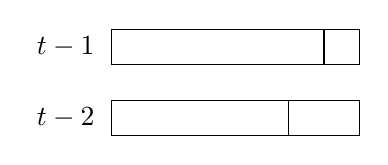
\begin{tikzpicture}[scale=0.45]
\draw (0,0) rectangle (6,1); \draw (6,0) rectangle (7,1); \node[left] at (-0.2,0.5) {$t-1$};
\draw (0,-2) rectangle (5,-1); \draw (5,-2) rectangle (7,-1); \node[left] at (-0.2,-1.5) {$t-2$};
\end{tikzpicture}
\end{center}

Given exactly $k$ ones in a word of length $\ell$, we are inserting $k$ ones into a sequence of $\ell-k$ zeros,
\[
{}_{\wedge}0_{\wedge}0_{\wedge}0_{\wedge}\cdots{}_{\wedge}0_{\wedge},
\]
at most one into each of the $\ell-k+1$ slots. So for each $k$ there are $\dbinom{\ell-k+1}{k}$ choices of order. \added{(Summing over $k$ gives $\sum_k\binom{\ell-k+1}{k}=F_{\ell+2}$.)}

So if the length of a ``$1$'' is $2$ and that of a ``$0$'' is $L$, the configuration with word of length $\ell$ \added{(i.e.\ $\ell+1$ discs)} containing $k$ ones has length
\[
t=2k+(\ell-k)L+2,
\]
the $+2$ coming from the two ends.

\begin{remark}
\unclear{Check: with open ends, a $1$ in the first or last slot seems not locally length-minimizing.}
\added{With truly open ends, an end disc lying against the same wall as its neighbour can roll around that neighbour towards the opposite wall, shortening $t$. If such end configurations are excluded, the count becomes $\binom{\ell-k-1}{k}$ instead of $\binom{\ell-k+1}{k}$; the asymptotics below are unchanged.}
\end{remark}

We can also compute the maximum of $\binom{n-k+1}{k}$ over $k$ (with $n=\ell$): as $n\to\infty$ the maximizing $k$ satisfies
\[
\frac kn\longrightarrow\frac5{10}-\frac{\sqrt5}{10}=\frac12-\frac{\sqrt5}{10}\approx0.276 .
\]
\begin{addedblock}
Indeed, with $x=k/n$, Stirling gives $\frac1n\ln\binom{n-k+1}{k}\to g(x)=(1-x)\ln(1-x)-x\ln x-(1-2x)\ln(1-2x)$, and $g'(x)=0$ becomes $(1-2x)^2=x(1-x)$, i.e.\ $5x^2-5x+1=0$, whose root in $(0,\tfrac12)$ is $x=\frac{5-\sqrt5}{10}$. At this point $g(x)=\ln\varphi$, $\varphi=\frac{1+\sqrt5}2$, which matches the growth $F_{n+2}\sim\varphi^{n}$: the maximal term carries the whole exponential growth.
\end{addedblock}

And there is a ``unique'' densest packing: \added{the zigzag with all contacts at opposite walls (the word $00\cdots0$, length $\ell L+2$), unique up to reflection. At the other extreme the least dense jammed configuration alternates pairs on the two walls (word $0101\cdots$, or $1010\cdots$ with ends allowed).}
\unclear{Second sketch annotated ``$\leftarrow$ \ldots\ last \ldots\ as well'': read as the least dense case.}

\begin{center}
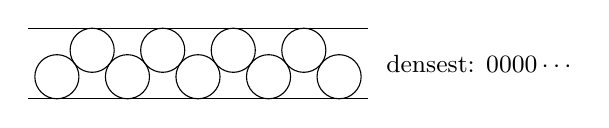
\begin{tikzpicture}[scale=0.28]
\draw (-1.3,0)--(14.1,0); \draw (-1.3,3.2)--(14.1,3.2);
\foreach \i in {0,...,8} { \pgfmathsetmacro{\y}{mod(\i,2)==0 ? 1 : 2.2} \draw (1.6*\i,\y) circle (1); }
\node[right] at (14.5,1.6) {\small densest: $0000\cdots$};
\end{tikzpicture}

\vspace{1ex}
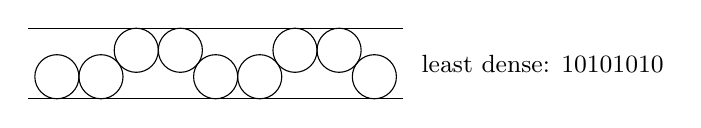
\begin{tikzpicture}[scale=0.28]
\draw (-1.3,0)--(15.7,0); \draw (-1.3,3.2)--(15.7,3.2);
\foreach \x/\y in {0/1,2/1,3.6/2.2,5.6/2.2,7.2/1,9.2/1,10.8/2.2,12.8/2.2,14.4/1} { \draw (\x,\y) circle (1); }
\node[right] at (16.1,1.6) {\small least dense: $10101010$};
\end{tikzpicture}
\end{center}

\begin{exercise}\label{L11:ex:typical}
Using the law of large numbers and \added{Stirling's} approximation, show that \added{if all jammed configurations of $n+1$ discs are equally likely (Edwards' ansatz without the volume constraint),} a typical configuration has a fraction
\[
\frac12-\frac{\sqrt5}{10}
\]
of $1$'s. \added{Deduce that its length per disc is close to $2x+(1-x)L$ with $x=\frac12-\frac{\sqrt5}{10}$.} Compare to coin flips, where the fraction would be $\tfrac12$.
\end{exercise}
\orig{``Ex.\ law of large \ldots\ \& approx.\ \ldots''; partly illegible}

\subsection{Outlook}
\begin{itemize}
\item Probabilities of critical points. \unclear{First word unclear (``prune''? ``prior''?).} Flow to jammed configurations\ldots\ The resulting distribution is probably concentrated on the maxima, since critical saddles should have probability near $0$. \added{(A saddle attracts only a lower-dimensional set of starting configurations under the flow.)}
\item $\Longrightarrow$ Question: compute these values!
\item Also\ldots\ for large $N$ this is hard, so we study low-order cases.
\end{itemize}
\unclear{last line read as ``so study low order cases''}
